\section{Working Process }
The workflow diagram in Figure 3.1 below shows an overview of each step to train, test, and validate our models.\\
 
First of all, we will collect our data sets. Then we will do data preprocessing through scaling, normalization, resizing, and augmentation. After finishing preprocessing, we will split our dataset into an 8:2 ratio. in which 80\% of the data set will be for training our model and 20\% will be for testing. After that, we will be doing feature extraction methods like Mel Spectrogram, MFCCs, and Wavelet. We will also take raw data to analyze our results. Then, through several neural network models like CNN and LSTM, we will train our model. After that, we will do a comparison to find the validation accuracy of our model. From the comparison, we will select some top Neural Network models that will result in the highest accuracy and add them to get more precise results. Finally, we will reach a conclusion based on the results of our model. 
\section{Used Feature Extractions and Architectures  }
    \subsection{Mel Spectrogram}
    The Mel Spectrogram is a visual representation of sound waves in which frequency and intensity are represented by the x-axis and y-axis, respectively. In it, time appears on the x-axis while various frequencies of sound appear on the y-axis. The different colors represent different intensity levels or frequencies of sound. CNN-LSTM achieves an accuracy of 64.58\% with MFCC features and ResNet-LSTM achieves an accuracy of 62.5\% using log-Mel spectrograms \parencite{16}. We took samples of air pressure over time to digitally represent an audio signal. We mapped the audio signal from the time domain to the frequency domain using the fast Fourier transform, and we performed this on overlapping windowed segments of the audio signal. We converted the y-axis (frequency) to a log scale and the color dimension (amplitude) to decibels to form the spectrogram. We mapped the y-axis (frequency) onto the mel scale to form the mel spectrogram. The audio signal goes to framing and transforms through Discrete Fourier. After mel filterbank and log, the audio is extracted and transformed as a Mel Spectrogram. 
            \begin{figure}[ht]
            \centering
            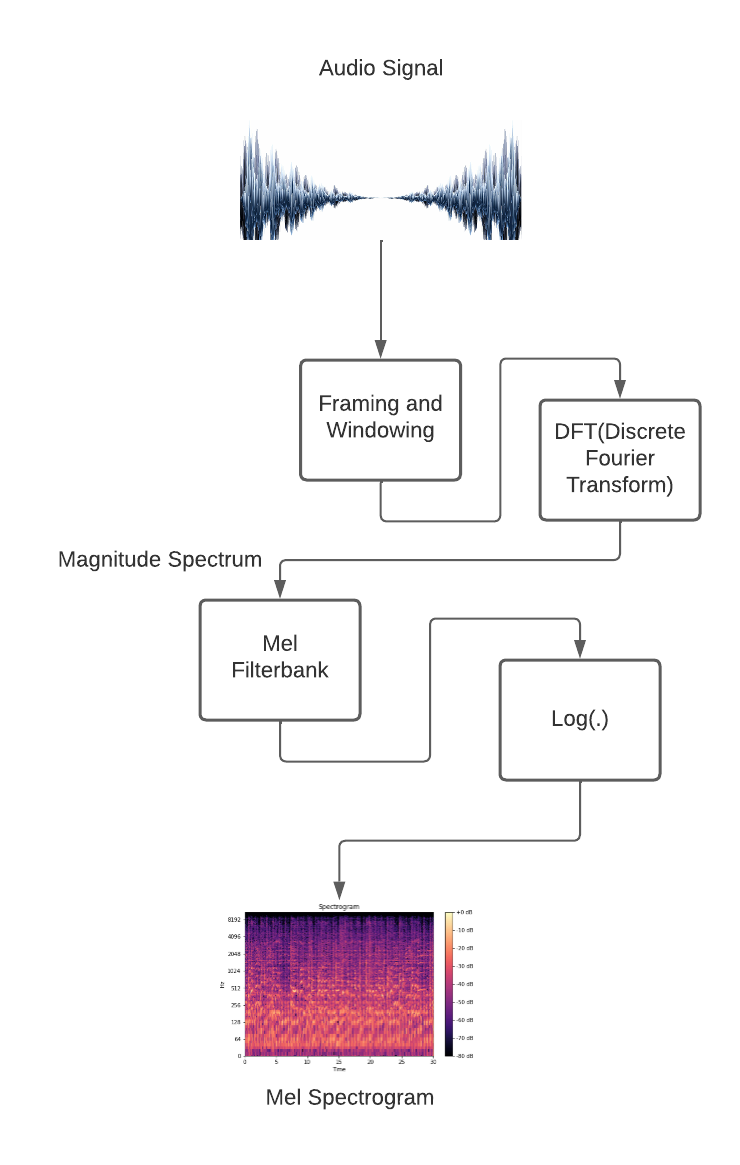
\includegraphics[scale=0.5]{images/figure1.png}
            \caption{Block diagram of Mel spectrogram of an audio signal.}
            \label{fig: Mel Spectrogram}
            \end{figure}
    \subsection{Wavelet}
    The Fourier transform is a useful tool to analyze the frequency components of the signal.  Wavelet transforms are based on small wavelets with limited duration. The translated-version wavelets locate where we concern. Whereas the scaled-version wavelets allow us to analyze the signal in different scale.
    \subsection{MFCC}
    Mel Frequency Cepstral Coefficients (MFCC), The Cepstral coefficients are the inverse-fft of the log of the spectrum; The MFCC are the inverse-fft of the log of the frequency-warped spectrum. The idea of MFCC is to convert audio in time domain into frequency domain so that we can understand all the information present in speech signals. MFCC is to convert time domain signals into frequency domain signal by mimicking cochlea function using Mel filters.
        \begin{figure}[ht]
        \centering
        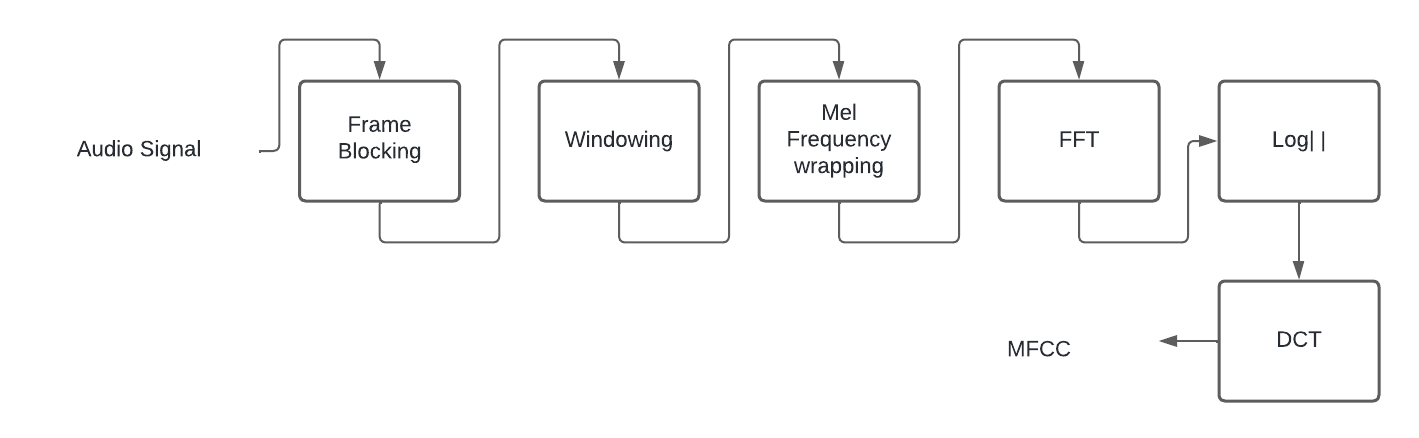
\includegraphics[scale=0.48]{images/figure2.png}
        \caption{Block diagram of MFCC.}
        \label{fig:x Block diagram of MFCC.}
        \end{figure}
    
    \subsection{CNN}
    A convolution tool that separates and identifies the various features of the audio for analysis in a process called "feature extraction." The network of feature extraction consists of many pairs of convolutional or pooling layers. A fully connected layer that utilizes the output from the convolution process and predicts the class of the audio based on the features extracted in previous stages. This CNN model of feature extraction aims to reduce the number of features present in a dataset. It creates new features which summarize the existing features contained in an original set of features. There are many CNN layers, as shown in the CNN architecture diagram.
    \begin{figure}[ht]
        \centering
        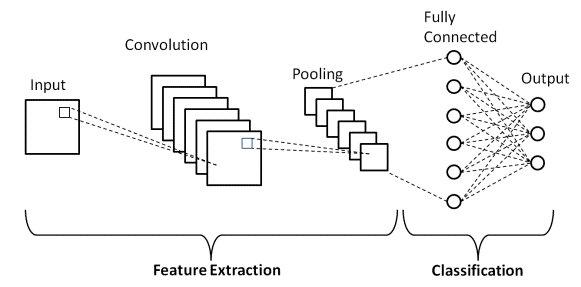
\includegraphics[scale=1]{images/figure3.png}
        \caption{Block diagram of CNN.}
        \label{fig:x Block diagram of CNN.}
        \end{figure}
    \subsection{LSTM}
    Aside from singular data points like photos, LSTM has feedback connections, making it capable of processing the complete sequence of data. This has uses in machine translation and speech recognition, among others. A unique version of RNN called LSTM exhibits exceptional performance on a wide range of issues.
